% Created 2019-11-03 Sun 19:20
% Intended LaTeX compiler: pdflatex
\documentclass[presentation]{beamer}
\usepackage[utf8]{inputenc}
\usepackage[T1]{fontenc}
\usepackage{graphicx}
\usepackage{grffile}
\usepackage{longtable}
\usepackage{wrapfig}
\usepackage{rotating}
\usepackage[normalem]{ulem}
\usepackage{amsmath}
\usepackage{textcomp}
\usepackage{amssymb}
\usepackage{capt-of}
\usepackage{hyperref}
\usepackage{listings}
\usepackage[backend=bibtex]{biblatex}
\bibliography{References}
\usepackage{amsmath, amssymb}
\usetheme{Boadilla}
\author{Curtis d'Alves, Nhan Thai, Nassim Khoonkari, \\ Padma Pasupathi, Tanya Bouman, Christopher Anand}
\date{November 6, 2019}
\title{Two Functional MDD's for the Price of One - Part 2}
\hypersetup{
 pdfauthor={TODO add list of authors},
 pdftitle={Two Functional MDD's for the Price of One - Part 2},
 pdfkeywords={},
 pdfsubject={},
 pdfcreator={Emacs 26.3 (Org mode 9.2.3)}, 
 pdflang={English}}
\lstdefinelanguage{AMPL}{keywords={set,param,var,arc,integer,minimize,maximize,subject,to,node,sum,in,Current,complements,integer,solve_result_num,IN,contains,less,suffix,INOUT,default,logical,sum,Infinity,dimen,max,symbolic
    ,Initial,div,min,table,LOCAL,else,option,then,OUT,environ,setof ,union,all,exists,shell_exitcodeuntil,binary,forall,solve_exitcodewhile ,by,if,solve_messagewithin,check,in,solve_result
  },sensitive=true,comment=[l]{\#}}
\definecolor{mGreen}{rgb}{0,0.6,0}
\definecolor{mGray}{rgb}{0.5,0.5,0.5}
\definecolor{mPurple}{rgb}{0.58,0,0.82}
\definecolor{backgroundColour}{rgb}{0.95,0.95,0.92}

\lstdefinestyle{CStyle}{
  backgroundcolor=\color{backgroundColour},   
  commentstyle=\color{mGreen},
  keywordstyle=\color{magenta},
  numberstyle=\tiny\color{mGray},
  stringstyle=\color{mPurple},
  basicstyle=\footnotesize,
  breakatwhitespace=false,         
  breaklines=true,                 
  captionpos=b,                    
  keepspaces=true,                 
  numbers=left,                    
  numbersep=5pt,                  
  showspaces=false,                
  showstringspaces=false,
  showtabs=false,                  
  tabsize=2,
  language=C
}
\lstdefinestyle{Haskell}{
  backgroundcolor=\color{backgroundColour},   
  commentstyle=\color{mGreen},
  keywordstyle=\color{magenta},
  numberstyle=\tiny\color{mGray},
  stringstyle=\color{mPurple},
  basicstyle=\footnotesize,
  breakatwhitespace=false,         
  breaklines=true,                 
  captionpos=b,                    
  keepspaces=true,                 
  numbers=left,                    
  numbersep=5pt,                  
  showspaces=false,                
  showstringspaces=false,
  showtabs=false,                  
  tabsize=2,
  language=haskell 
}
\begin{document}

\maketitle
\begin{frame}{Outline}
\tableofcontents
\end{frame}


\section{Symphony - Syntax Guide Part 1}
\label{sec:org5ab5078}
\begin{frame}[label={sec:org5cb1731}]{Symphony - Modeling Language for Non-Linear Optimization}
\begin{itemize}
\item Models linear and non-linear optimization problems
\item Simple declarative language
\item Support for bounded parameters and constraint programming
\item Generates performance oriented c code
\item Solver Agnostic (plug into your solver of choice)
\end{itemize}
\end{frame}

\begin{frame}
  \frametitle{Vectors and dimension}
  \begin{itemize}
    \item In Symphony, everything is vector.
    \item Vectors
      \begin{itemize}
    \item Dimension (Shape): can be scalar, 1D, 2D, 3D, ...
      \begin{itemize}
      \item Scalar is just a single number 
      \item 1D(n) variable is an array of n number, useful for problems in signal processing, sound processing, ..
      \item 2D(m x n) variable is a 2D array of m x n numbers, useful for problems in image processing, ...
      \item 3D(m x n x p) variable is a 3D array of m x n x p numbers, useful for
        problems in topology, image processing with voxels, ...
      \end{itemize}
    \item Numtype: can be real (R) or complex (C)
      \end{itemize}
    \item We can manipulate vectors like adding, multiplying, doing inner product, ... to form new vectors (expressions).
  \end{itemize}
\end{frame}

\begin{frame}[fragile]
  \frametitle{Forming An Expression}

  \begin{itemize}
    \item $(+),(-),(*),(/)$ Add/Subtract/Multiply/Divide (point-wise) two vectors having same shape and same numtype
    \item $(*.)$ Scale a vector with a scalar (if they form a vector space in Mathematics, i.e, real number can scale anything, 
    but complex can only scale complex)
    \item $(\textsc{<.>})$ Inner product (dot product) of two vectors 
    \item (\^{}) Power a vector with an integer
    \item Piecewise:
    \begin{lstlisting}[style=Haskell]
    case x:
      x <= 0    -> -x
      otherwise -> x
    \end{lstlisting} 
    \item sumElements, norm2square, normHuber
  \end{itemize}
\end{frame}

% TODO add formal defintions for sumElements, norm2square, normHuber

\begin{frame}[fragile]
  \frametitle{Structure}
  A valid symphony problem consists of:
  \begin{itemize}
  \item Variables 
  \item Objective function 
  \item Constants (optional)
  \item Constraints (optional)
  \end{itemize}
\end{frame}

\begin{frame}[fragile]
  \frametitle{Variable Declaration}

  \begin{itemize}
  \item Variables are declared in a {\color{red} variable} block
  \item For example:
  \begin{lstlisting}[style=Haskell]
  variables:
    x[100][100] = 10
    y[20][20][20]
    a, b = 2, c
  \end{lstlisting}
  \item Assignment denotes an initial value
  \item Unassigned variables will be randomly iniatlized witha number between (0,1)
  \end{itemize}
\end{frame}

\begin{frame}[fragile]
  \frametitle{Objective Function}

  \begin{itemize}
  \item Declared in a {\color{red} minimize} block
  \item For example:
  \begin{lstlisting}[style=Haskell]
  minimize:
    (x - y)^2
  \end{lstlisting}
  \item Must evaluate to a scalar (one dimensional value)
  \end{itemize}
\end{frame}

\begin{frame}[fragile]
  \frametitle{Constant Declarations}

  \begin{itemize}
  \item Declared in a {\color{red} constants} block
  \item For example:
  \begin{lstlisting}[style=Haskell]
  constants:
    m = 2
    delta = 10, sigma = 15
    mask[100][100] = Pattern(FIRST_ROW_1)
  \end{lstlisting}
  \item Unlike variables, cosntants must be assigned, and are not optimized over
  \item Multi-dimensional constants can be assigned using the Pattern function,
    which takes the following macros as input
  \begin{lstlisting}[style=CStyle]
    FIRST_COLUMN_0, FIRST_COLUMN_1, LAST_ROW_0
    LAST_ROW_1, LAST_COLUMN_0, LAST_COLUMN_1 ...
  \end{lstlisting}
  \end{itemize}
\end{frame}

\begin{frame}[fragile]
  \frametitle{Local Variables}

  \begin{itemize}
    \item Sometimes your expression can become to convoluted, declare local
      variables using a {\color{red}let} block
    \item For example:
  \begin{lstlisting}[style=Haskell]
  let:
    regularizerX = norm2square x
    regularizerY = norm2square y
    regularizer = regularizerX + regularizerY

  minimize:
    norm2square (x - y) + regularizer      
  \end{lstlisting}
  \end{itemize}
\end{frame}
\section{Sample Problem 1}
\label{sec:org94a0e83}
\begin{frame}[label={sec:org802260d}]{Sample Problem 1 - Velocity Problem}
\begin{center}
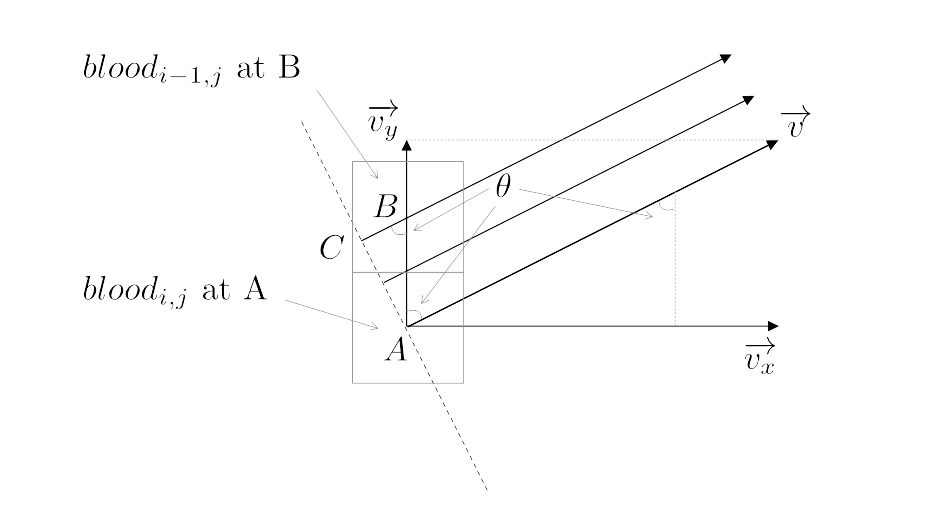
\includegraphics[width=8cm]{figs/velocity.png}
\end{center}
\begin{itemize}
\item MRI imaging problem dealing with blood flow
\item Given vector field of blood flow: can we find how long each blood cell has been there?
\item Do this by minimizing the \alert{flow} over time (hence an optimization problem!)
\end{itemize}
\end{frame}

\begin{frame}[label={sec:org03d5ffb}]{Velocity Problem - Model Derivation}
\begin{center}
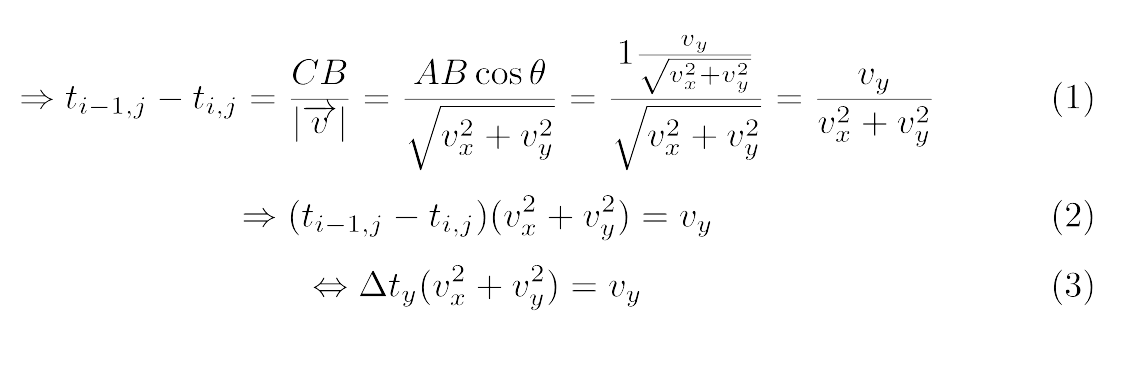
\includegraphics[width=.9\linewidth]{figs/velocityderivation.png}
\end{center}
\end{frame}
\begin{frame}[label={sec:org06e74f7}]{Velocity Problem - Optimization Model}
\begin{align*}
\min_t &\sum_{\textsc{pixels}} (\Delta t_x (v_x^2 + v_y^2) - v_x) * v_x^2)^2  \\
               & + \sum_{\textsc{pixels}} (\Delta t_y ((v_x^2 + x_y^2) - x_y) * x_y^2)^2 \\
v_{(x,y)} \quad & \textsc{velocity in x,y direction} \\
t_{(x,y)} \quad & \textsc{time in x,y direction}
\end{align*}
\end{frame}

\section{Symphony - Syntax Guide Part 2}

% TODO add frame on Complex numbers
\begin{frame}[fragile]
  \frametitle{Variable Bounds}
  \begin{itemize}
  \item Variable bounds are put in a {\color{red} constraints} block
  \item For example:
  \begin{lstlisting}[style=Haskell]
  constants:
    yUpperBound = 5  
  constraints:
    x >= 10
    y <= yUpperBound
  \end{lstlisting}
  \item Bounds must be assigned to a value or constant (not an expression)
  \end{itemize}
\end{frame}

\begin{frame}[fragile]
  \frametitle{File Storage}

  \begin{itemize}
    \item Values for variabels or constants can be loaded from text files or
      HDF5 datasets
    \item For example:
  \begin{lstlisting}[style=Haskell]
  constants:
    b[10][10] = File("b.txt")
  variables:
    real[128][128] = Dataset("dataset.hd5","real")
    imag[128][128] = Dataset("dataset.hd5","imag")
  \end{lstlisting}
  \end{itemize}
\end{frame}

\begin{frame}
  \frametitle{HDF5 - Hierarchical Data Format}
  \begin{itemize}
  \item Designed to store and organize large amounts of data
  \item Capable of storing multiple labeled datasets in a single file
  \item Great library {\color{blue}h5py} for python, capable of generating data
    straight from numpy arrays
  \end{itemize}
\end{frame}
\section{Sample Problem 2}
\label{sec:org0fb732f}
\begin{frame}[label={sec:org0ee1152}]{Brain Problem - 1}
\begin{center}
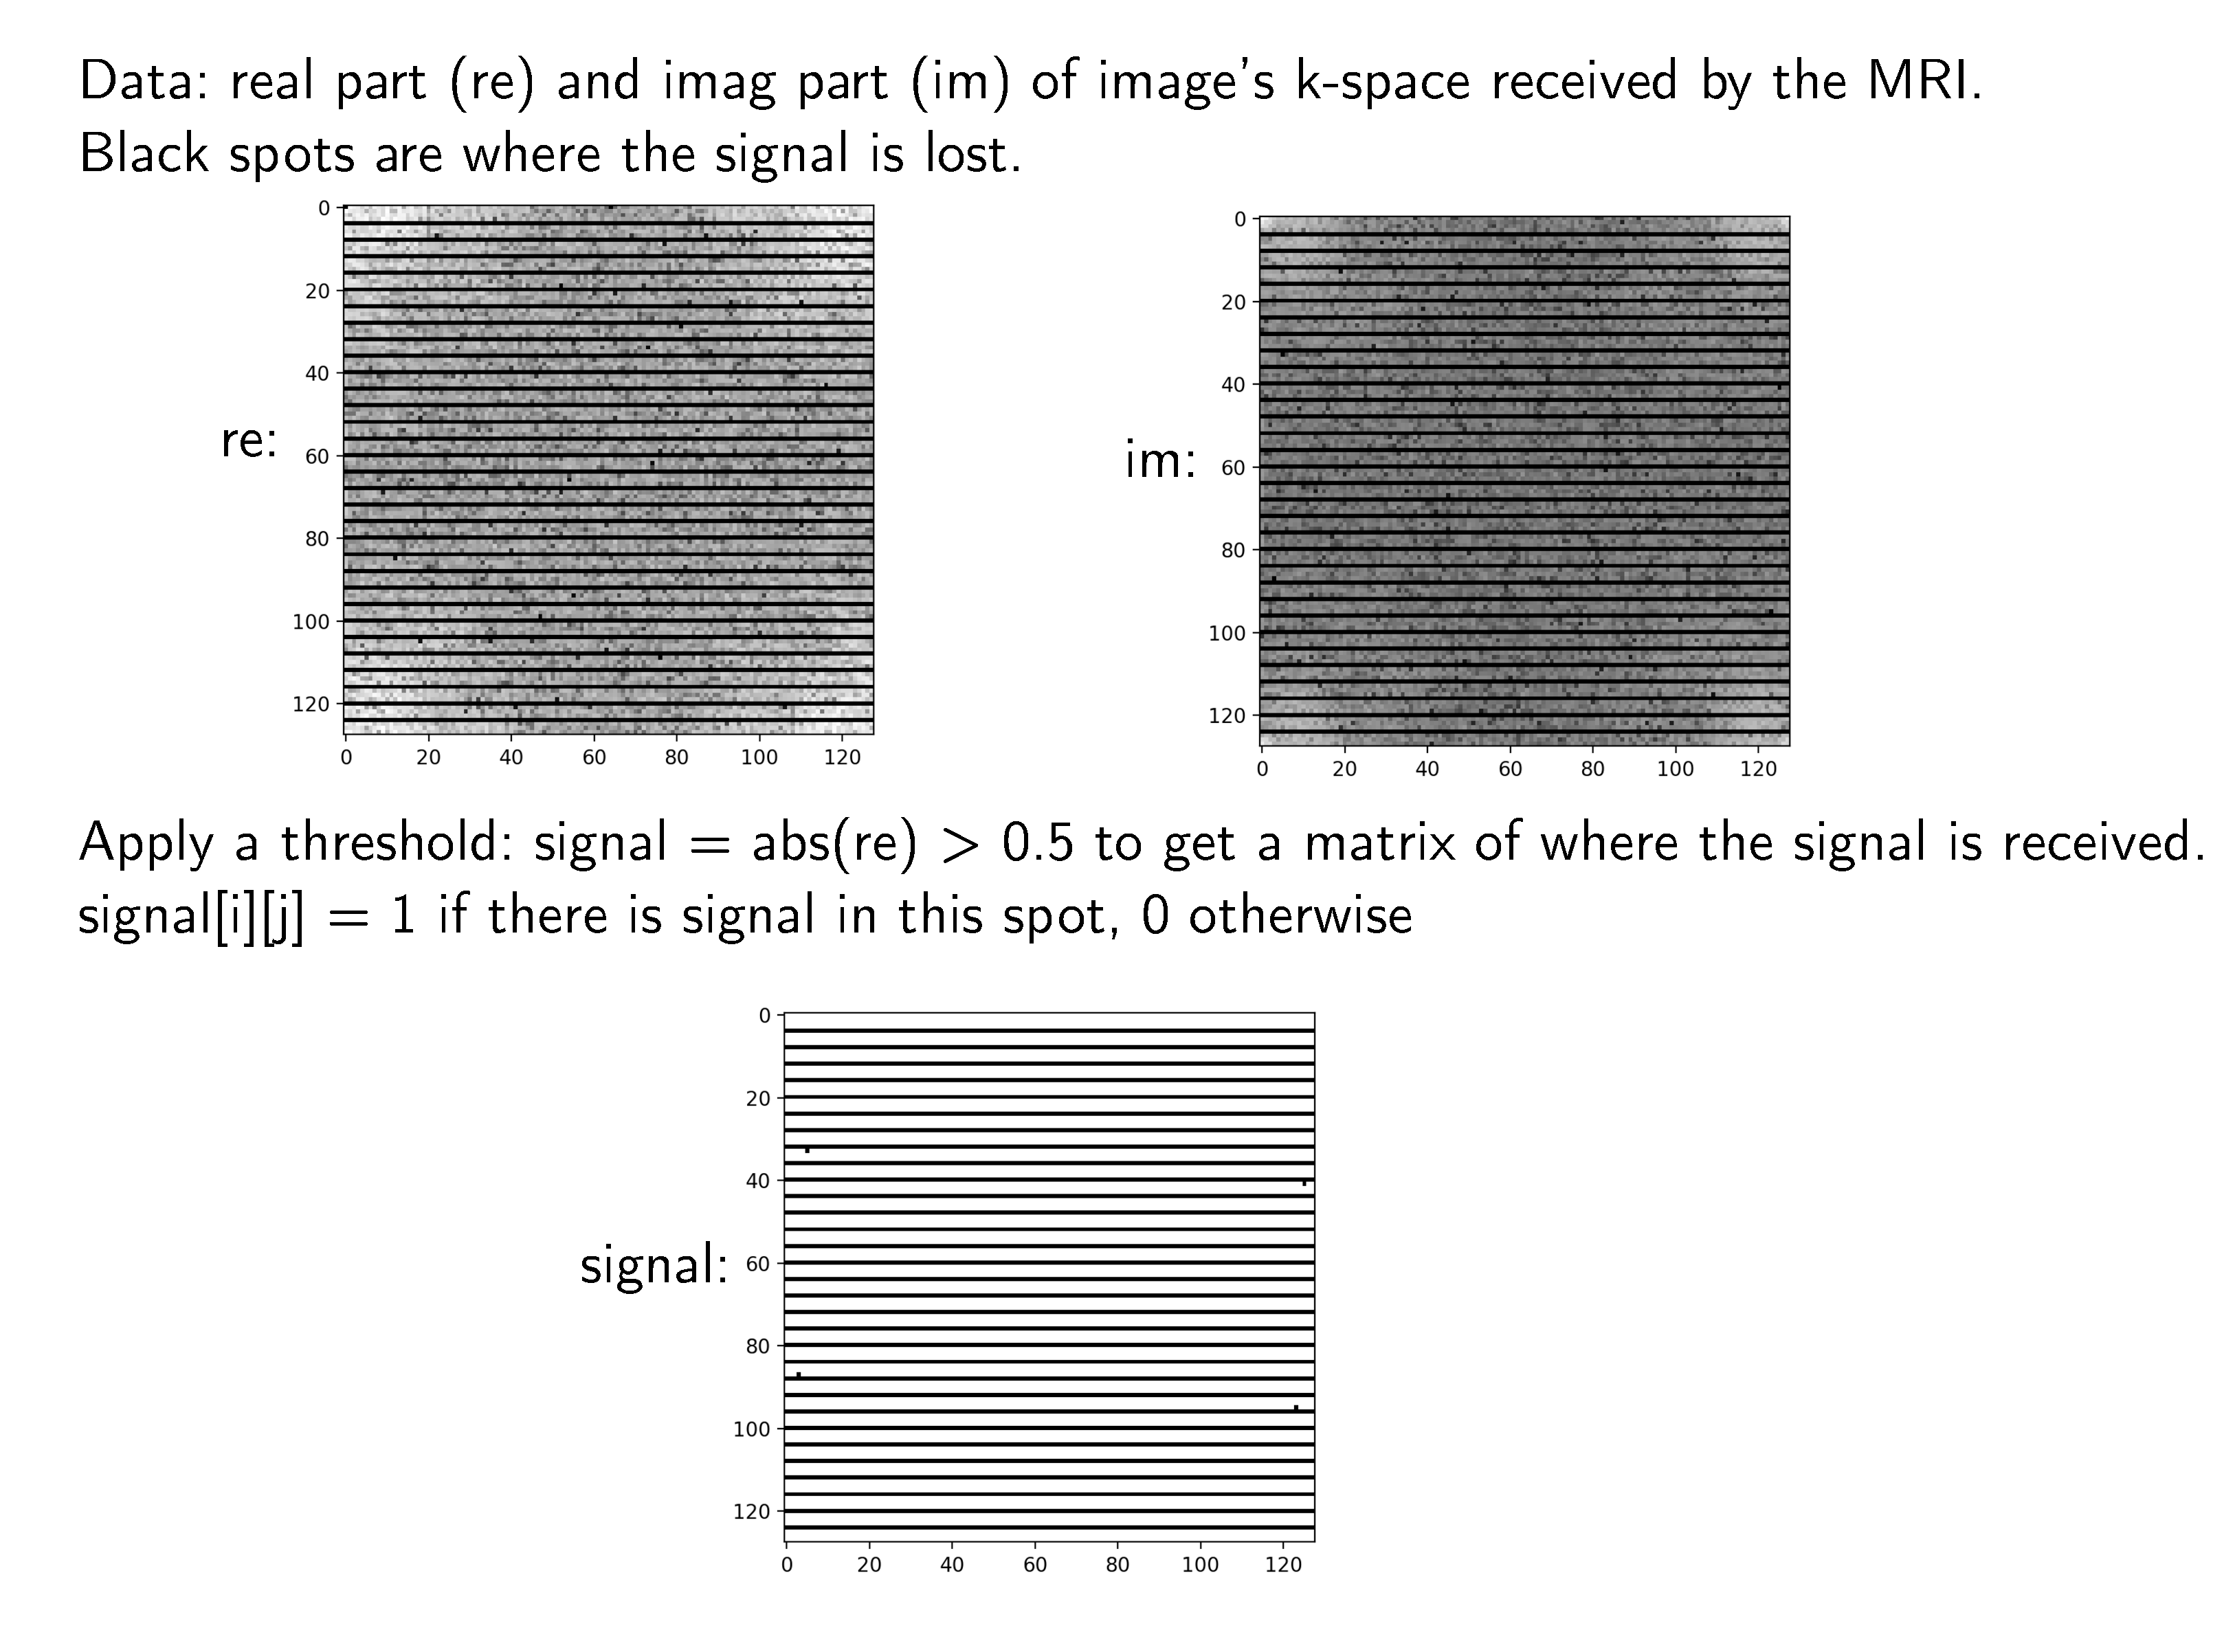
\includegraphics[width=.9\linewidth]{figs/MRIBrain1.pdf}
\end{center}
\end{frame}

\begin{frame}[label={sec:org2a77819}]{Brain Problem - 2}
\begin{center}
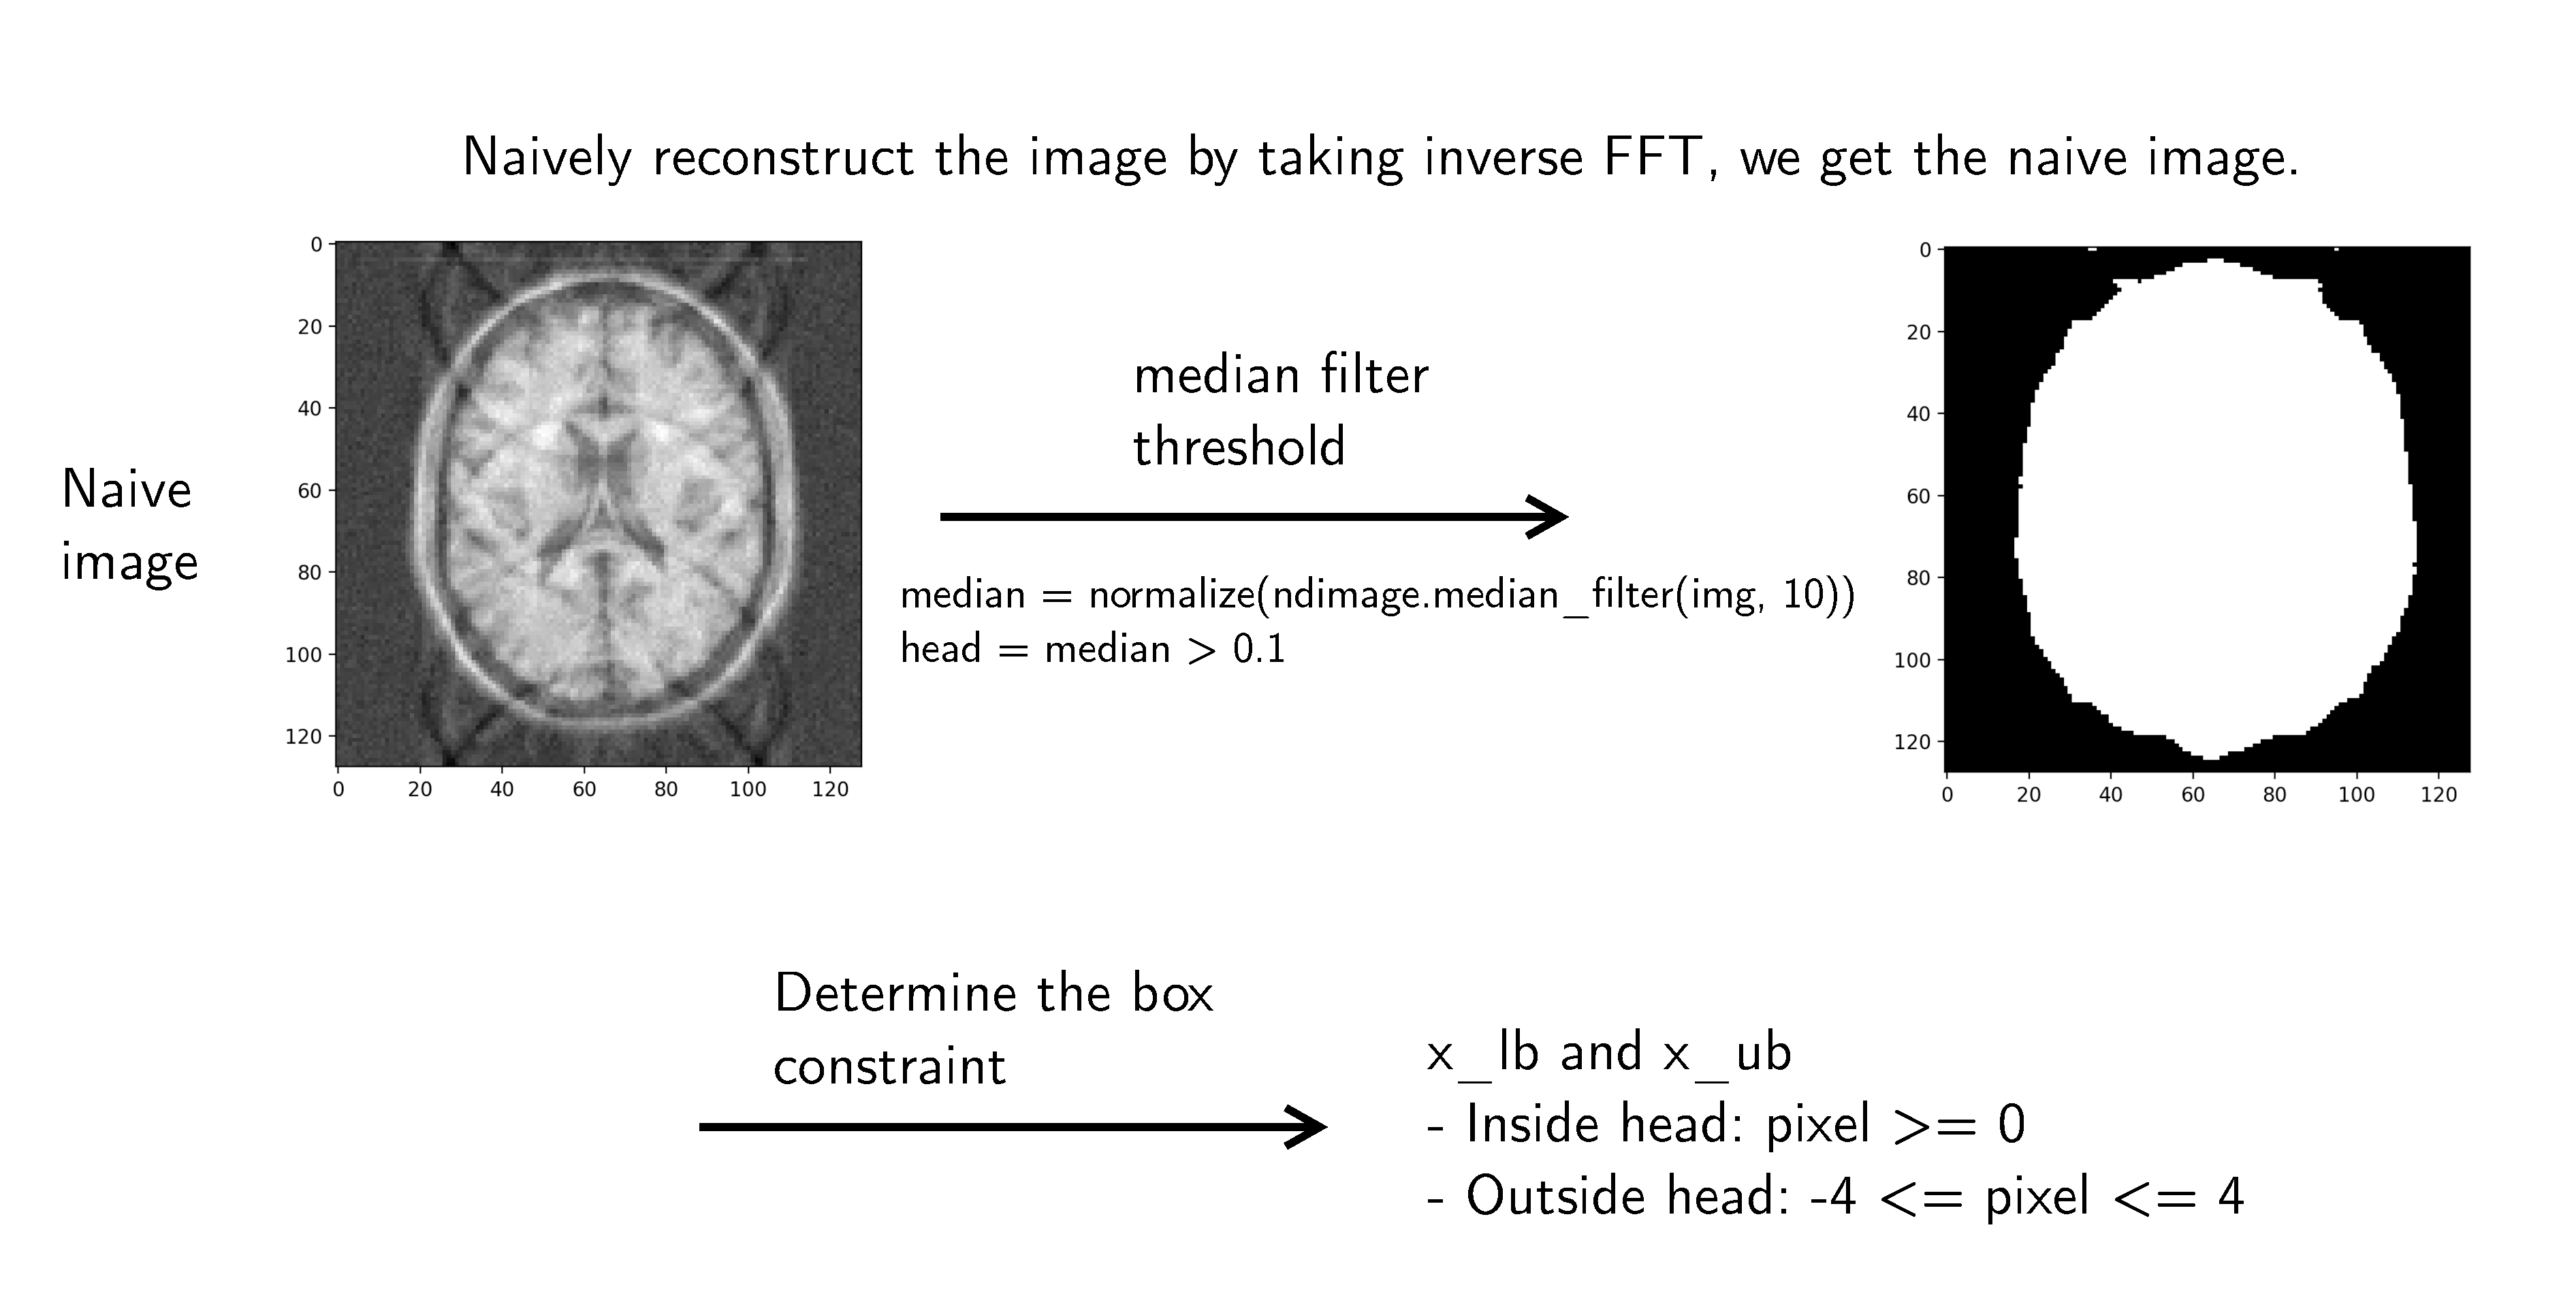
\includegraphics[width=.9\linewidth]{figs/MRIBrain2.pdf}
\end{center}
\end{frame}

\section{Sample Problem 3}
\begin{frame}
  \frametitle{Multi-Coil MRI}

  \begin{align*}
    \min \limits_{\rho} &\sum \limits_{i=0}^{\textsc{\#coils}} || FT(P))-m_i||^2 \\
                             &+ \lambda (||\delta_x (\rho) ||^2 + || \delta_y(\rho) ||^2) \\
  \end{align*}
  
  \begin{align*}
    \rho &= \textsc{ True Image} \\
    S_i &= \textsc{ Coil Sensitivity} \\
    m_i &= \textsc{ K-Space measurement } \\
    \lambda &= \textsc{ scaling }
  \end{align*}

\end{frame}
% TODO add pictures of individual coils
\section{Symphony - Syntax Guide Part 3}

\begin{frame}[fragile]
  \frametitle{Constraints}

  \begin{itemize}
  \item Declared in a {\color{red} constraints} block (just like variable bounds)
  \item For example:
  \begin{lstlisting}[style=Haskell]
  constraints:
    x <.> x >= 0  
  \end{lstlisting}
  \item Expression must be on LHS and must evaluate to scalar (one-dimensional value)
  \item {\bf Note}: limits your choice of supported solvers 
  \end{itemize}
\end{frame}

\section{Sample Problem 4}
% TODO cleanup logistics problem
\begin{frame}[fragile]
 \frametitle{Logistics Problem} 
  \begin{itemize}
    \item In most logistic problems we want to Maximize the benefits or Minimize the costs.
      \item This table is for defining the revenue of sending products from factories to companies.

  \begin{center}
    \begin{tabular}{ c | c | c }
      & Company1 & Company2 \\ \hline
      Factory1 & 1.75 & 2.25 \\  
      Factory2 & 2.00 & 2.50    
    \end{tabular}
  \end{center}

  \item the below table shows the demand of companies. Also the capacity of each factory for producing is 60000.


  \begin{center}
    \begin{tabular}{ c | c | c }
      & Company1 & Company2 \\ \hline
      Factory1 & $x_{11}$ & $x_{12}$ \\  
      Factory2 & $x_{21}$ & $x_{22}$ \\
      &23000 & 30000    
    \end{tabular}
  \end{center}
  \end{itemize}
\end{frame}

\begin{frame}
  \frametitle{Logistics Problem}
 \begin{itemize} 
  \item we want to Maximize the revenue.\\
  \begin{center}
    $Max f(x) =  Min - f(x)$
  \end{center}

  \item So we will have:\\
  \begin{center}
    $Min  -((c_{11} * x_{11}) + (c_{12} * x_{12}) + (c_{21} * x_{21}) + (c_{22} * x_{22}) )$\\

    subject to:\\

    $x_{11} \geq 0$, $ x_{12} \geq 0$,  $ x_{21} \geq 0$,   $ x_{22} \geq 0$\\
    $x_{11}+x_{21} \geq$ DemandCompany1\\
    $x_{12}+x_{22} \geq$ DemandCompany2\\
    $x_{11}+x_{12} \leq$ CapacityFactory1\\
    $x_{21}+x_{22} \leq$ CapacityFactory2\\
  \end{center}
  \end{itemize}
\end{frame}

\begin{frame}
  \frametitle{Logistics Problem}
  variables here are the the products which are sent from each factory to each company.\\
 
  \begin{center}
    CapacityFactory1 = 600000\\
    CapacityFactory2 = 600000\\

    DemandCompany1 = 30000\\
    DemandCompany2 = 23000\\
    $c_{11} \rightarrow$  revenue of $x_{11} = 1.75$\\
    $c_{12}  \rightarrow$  revenue of $x_{12} = 2.25$\\
    $c_{21} \rightarrow$  revenue of $x_{21} = 2$\\
    $c_{22} \rightarrow$ revenue of $x_{22} = 2.50$

  \end{center} 
\end{frame}
% \begin{frame}[label={sec:orgff6ee47}]{Play With L2-Norm / Hubar Penalty}
% \end{frame}

% \section{Hashed Expression - Symphony's Backend}
% \label{sec:org737f90f}
% \begin{frame}[label={sec:org4426ae4}]{Hashed Expression - Symphony's Backend}
% \begin{itemize}
% \item Embedded Language in \alert{Haskell}
% \end{itemize}
% \end{frame}

\end{document}